\section{Differencing}
\label{sec:pumpkin-diff}

% TODO organize into subsections
% TODO either include some algorithm, or include a note about why not

% From Motivating the Core, modified and augmented

Differencing is aware of and guided by the semantics of Coq's rich proof term language Gallina---that is, it is a \textit{semantic differencing} algorithm.
This means that differencing can take advantage of the structure and information carried in every proof term,
thanks to Gallina's rich type theory CIC$_{\omega}$.
The rich structure of terms helps guide differencing for each configuration,
while the rich information in their types helps ensure correctness in the end.

Consider once again the example from Figure~\ref{fig:example}, but this time not just the base case.
Both versions of the proof are inductive proofs using the same induction principle, with slightly different motives.
Accordingly, differencing knows that there are two places to look for candidates, namely the base case (line 13)
and the inductive case (line 14).
Differencing breaks each inductive proof into these cases, then recursively calls itself for each case.
In the base case, it finds the candidate from Section~\ref{sec:pumpkin-spec-diff}.
Since this candidate has the desired type for the configuration specialized to the base case, differencing knows it has successfully found a candidate.

The rich type information proof terms carry helps prevent exploration of syntactic differences that are not meaningful.
For example, in the inductive case of the proof term from Figure~\ref{fig:example} (line 14), the inductive hypothesis \lstinline{IHle} changes:

\begin{lstlisting}[language=coq]
  $\ldots$ (IHle : (@\diff{n <= m0 + 1}@)) $\ldots$(@\vspace{-0.08cm}@)
  $\ldots$ (IHle : (@\diff{n <= m0}@)) $\ldots$
\end{lstlisting}
Notably, though, the type of \lstinline{IHle} changes for \emph{any} two inductive proofs over \lstinline{le}
with different conclusions. A syntactic differencing component 
may identify this change as a candidate.
My semantic differencing algorithms know that they can ignore this change.
This section describes the design (Section~\ref{sec:pumpkin-diff-design}) and limitations (Section~\ref{sec:pumpkin-diff-limitations}) of these algorithms.
Section~\ref{sec:pumpkin-impl-diff} describes the implementation in \sysname.

\subsection{Design}
\label{sec:pumpkin-diff-design}

% TODO show examples, formalize if time!!!

Differencing recurses over the structure of two terms $t_A$ and $t_B$ in a common environment $\Gamma$.
When it recurses, it extends $\Gamma$ with common assumptions, then differences subterms.
In each case, it carries a goal type $G$, and returns a list of patch candidates $\vec{t}$ that each have that goal type.
That is, we can view it as a judgment $\Gamma\ \vdash\ (t_a,\ t_b,\ G) \Downarrow_{d} \vec{t}$,
where in the end, for every $t$ in $\vec{t}$, $\Gamma \vdash t : G$.

The details of this vary by the structure of the term and the configuration, with different heuristics corresponding to different subterm-configuration combinations.
For historical reasons, as \sysname was a prototype and differencing of proof terms was novel at the time, these heuristics are not formalized. % TODO formalize if time
Here I describe the design of some of the heuristics in CIC${_\omega}$.
Section~\ref{sec:pumpkin-impl-diff} describes additional features needed for implementation in Gallina,
and the \toolnamec extension in Chapter~\ref{chapt:pi} formalizes a more elegant differencing algorithm building on some of the insights from the \sysname differencing prototype.

\paragraph{Identity}
The simplest patch is the identity patch.
When two terms are definitionally equal, % TODO need to explain this somewhere, using latest text from PUMPKIN Pi
differencing infers that the goal is identity,
and returns a singleton list containing only the identity function instantiated to the appropriate type.

\paragraph{Application}
When one proof term is a function application, for example:

\begin{lstlisting}
  $\Gamma \vdash (f\ t_a,\ t_b,\ G) \Downarrow_{d} \vec{t}$
\end{lstlisting}
differencing checks to see if $t_b$ is in $f\ t_a$.
That is, it searches for a subterm of $f\ t_a$ that is definitionally equal to $t_b$.
This is how differencing can identify the candidate for the base case of Figure~\ref{fig:example} (line 13).
It is also a core building block that other differencing heuristics rely on.

When both proof terms are function applications, and the above heuristic fails:

\begin{lstlisting}
  $\Gamma \vdash (f_a\ t_a,\ f_b\ t_b,\ G) \Downarrow_{d} \vec{t}$
\end{lstlisting}
differencing may recurse into both the functions and the arguments, search for patches, and then compose the results.
How to compose those results varies by configuration.

\paragraph{Functions} % TODO in Chapter 2, need to mention hypos versus debruijn
The treatment of functions depends on whether a hypothesis or a conclusion has changed.
When recursing into the body of two functions, each with a hypothesis of the same type:

\begin{lstlisting}
  $\Gamma \vdash (\lambda (t_a : T) . b_a, \lambda (t_b : T) . b_b,\ G) \Downarrow_{d} \vec{t}$
\end{lstlisting}
differencing assumes that the conclusion has changed.
That is, it assumes that $t_a$ and $t_b$ are the same, adds one of them to a common environment,
and differences the body:

\begin{lstlisting}
  $\Gamma,\ t_a : T \vdash (b_a,\ b_b [t_a / t_b]) \Downarrow_{d} \vec{b}$
\end{lstlisting}
It then filters those candidates $\vec{b}$ to only those with an adjusted goal type $G\ t_a$,
then wraps each candidate $b$ in $\vec{b}$ in a function in the end:

\begin{lstlisting}
  $\lambda (t_a : T) . b$
\end{lstlisting}
with type $G$.

When a hypothesis type has changed:

\begin{lstlisting}
  $\Gamma \vdash (\lambda (t_a : T_a) . b_a, \lambda (t_b : T_b) . b_b,\ G) \Downarrow_{d} \vec{t}$
\end{lstlisting}
differencing acts similarly, but it substitutes the changed hypothesis type in the body in order to recurse into a well-typed environment.
It also has some additional logic to remove hypothesis that need not show up in the goal type.

\paragraph{Eliminators} % From implementation, plus some additional stuff
The semantic differencing algorithms views inductive types as \emph{trees} that represent their eliminators.
In these trees, every node is a type context, and every edge is an extension to that type context 
with a new term.\footnote{These trees are inspired by categorical models of dependent type theory~\cite{Hofmann97}.}
Correspondingly, type differencing (to identify goal types) compares nodes, 
and term differencing (to find candidates) compares edges. 

\begin{figure}[t]
\begin{center}
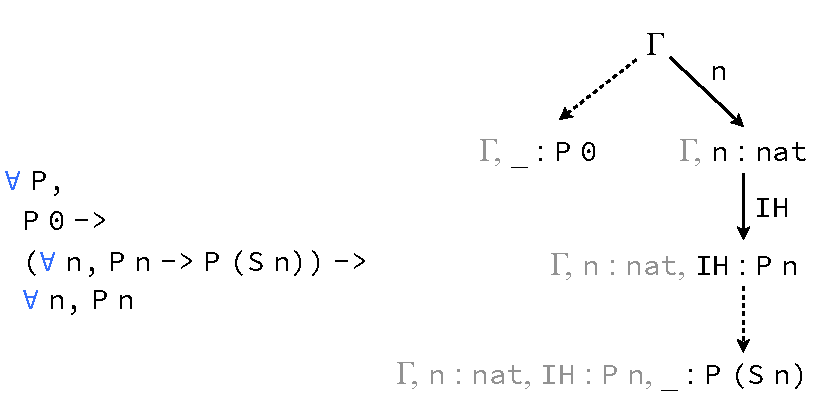
\includegraphics[scale=0.55]{repair/nat_ind}
\end{center}
\caption{The type of (left) and tree for (right) the eliminator of \lstinline{nat}. The solid edges represent hypotheses, and the dotted edges represent the proof obligations for each case in an inductive proof.} % TODO use Pi instead of forall
\label{fig:cattree}
\end{figure}

The key benefit to this model is that it provides a natural way to express inductive proofs, so
that differencing can efficiently identify good candidates.
Consider, for example, searching for a patch between conclusions of two inductive proofs of theorems about the natural numbers:

\begin{lstlisting}
  $Elim (nat,\ P)\ \{ f_O,\ f_S \}$
  $Elim (nat,\ Q)\ \{ g_O,\ g_S \}$ 
\end{lstlisting}
with goal type:

\begin{lstlisting}
  $Q \rightarrow P$
\end{lstlisting}

Differencing looks in both the base case and in the inductive case for candidates.
In each case, differencing diffs the terms in the dotted edges of the tree for the eliminator of \lstinline{nat} (Figure~\ref{fig:cattree}) to
try to find a term that maps between conclusions of that case:

\begin{lstlisting}[language=coq]
  $\Gamma \vdash (f_O,\ g_O,\ Q\ O \rightarrow P\ O) \Downarrow_{d} \vec{t_O}$
  $\Gamma \vdash (f_S,\ g_S,\ \Pi (n : nat) . Q\ (S\ n) \rightarrow P\ (S\ n)) \Downarrow_{d} \vec{t_S}$
\end{lstlisting}
In the inductive case, differencing also knows that the change in the type of the inductive hypothesis is not semantically relevant (it occurs for any change in the inductive motive).
Furthermore, it knows that the inductive hypotheis cannot show up in the patch itself, since the goal type does not reference the inductive hypothesis,
so it attempts to remove any occurrences of the inductive hypothesis in any candidate.

When differencing finds a candidate, it knows $Q$ and $P$ as well as the arguments $O$ or $S\ n$.
This makes it simple for \sysname to later query the transformations for the final patch, with type $Q \rightarrow P$.

\subsection{Limitations}
\label{sec:pumpkin-diff-limitations}

% Some from future work, some from us. Needs better framing.

This section describes a few fundamental limitations of differencing in \sysname,
and whether they are addressed in the later \toolnamec extension.
Limitations that are due to the choice of implementation strategy are in Section~\ref{sec:pumpkin-impl-diff}.

\paragraph{Heuristics}
Differencing in \sysname is heuristic-based.
This is to some degree inevitable, as the space of possible changes is infinite.
In particular, it is the cartesian product of the space of every possible old term and type,
combined with every possible new term and type.
Still, this is partly historical: for the \sysname prototype, the heuristics were designed bottom-up, and were in many cases too narrow or redundant.
The extension to differencing in \toolnamec not only supports a large class of changes not supported by \sysname,
but also abstracts many more details of heuristics.

\begin{figure*}[ht]
\begin{minipage}{0.48\textwidth}
\begin{lstlisting}[language=coq]
fun n m p (H : n <= m) (H0 : m <= p) =>(@\vspace{-0.04cm}@)
  (@\diff{le\_S n p}@) (* ... proof of stronger lemma *)(@\vspace{-0.04cm}@)
: (@\ltacforall@) n m p, n <= m -> m <= p -> n <= (@\diff{S p}@)
\end{lstlisting}
\end{minipage}
\hfill
\begin{minipage}{0.48\textwidth}
\begin{lstlisting}[language=coq]
fun n m p (H : n <= m) (H0 : m <= p) =>(@\vspace{-0.04cm}@)
  (@\diff{le\_plus\_trans n p 1}@) (* ... proof of stronger lemma *)(@\vspace{-0.04cm}@)
: (@\ltacforall@) n m p, n <= m -> m <= p -> n <= (@\diff{p + 1}@)
\end{lstlisting}
\end{minipage}
\vspace{-.35cm}
\caption{Two proof terms \lstinline{old} (left) and \lstinline{new} (right) that contain the same proof of a stronger lemma.}
\label{fig:stronger}
\end{figure*}

\paragraph{Isolating Changes} Differencing supports only incremental changes.
Proof engineers, in contrast, often make multiple changes to a verification project in the same commit. % TODO recall REPLICA somewhere, forward tease about later stuff on this
The challenge for differencing is to break down large, composite changes into small, isolated changes,
then use the appropriate heuristics.
Differencing cannot do this yet, and the later \toolnamec cannot do this either.
However, the user study made it clear that in real life, this would be very useful during development,
since proof engineers make much more granular changes in development time, % TODO all draft text
so this is less of an issue than I had originally expected it to be.
Still, change isolation would help with extracting repair benchmarks from artifacts, supporting library and version updates, and integrating with CI systems.
One idea for this is to draw on work in change and dependency management~\cite{873647, Autexier:2010:CMH:1986659.1986663, Celik:2017:IRP:3155562.3155588} to identify changes,
then use the factoring component to break those changes into smaller parts.


